\begingroup \pagestyle{empty}

\begin{titlepage} \thispagestyle{empty} \begin{tikzpicture}[remember picture, overlay]
\node[anchor=south west, inner sep=0] at (current page.south west) {%
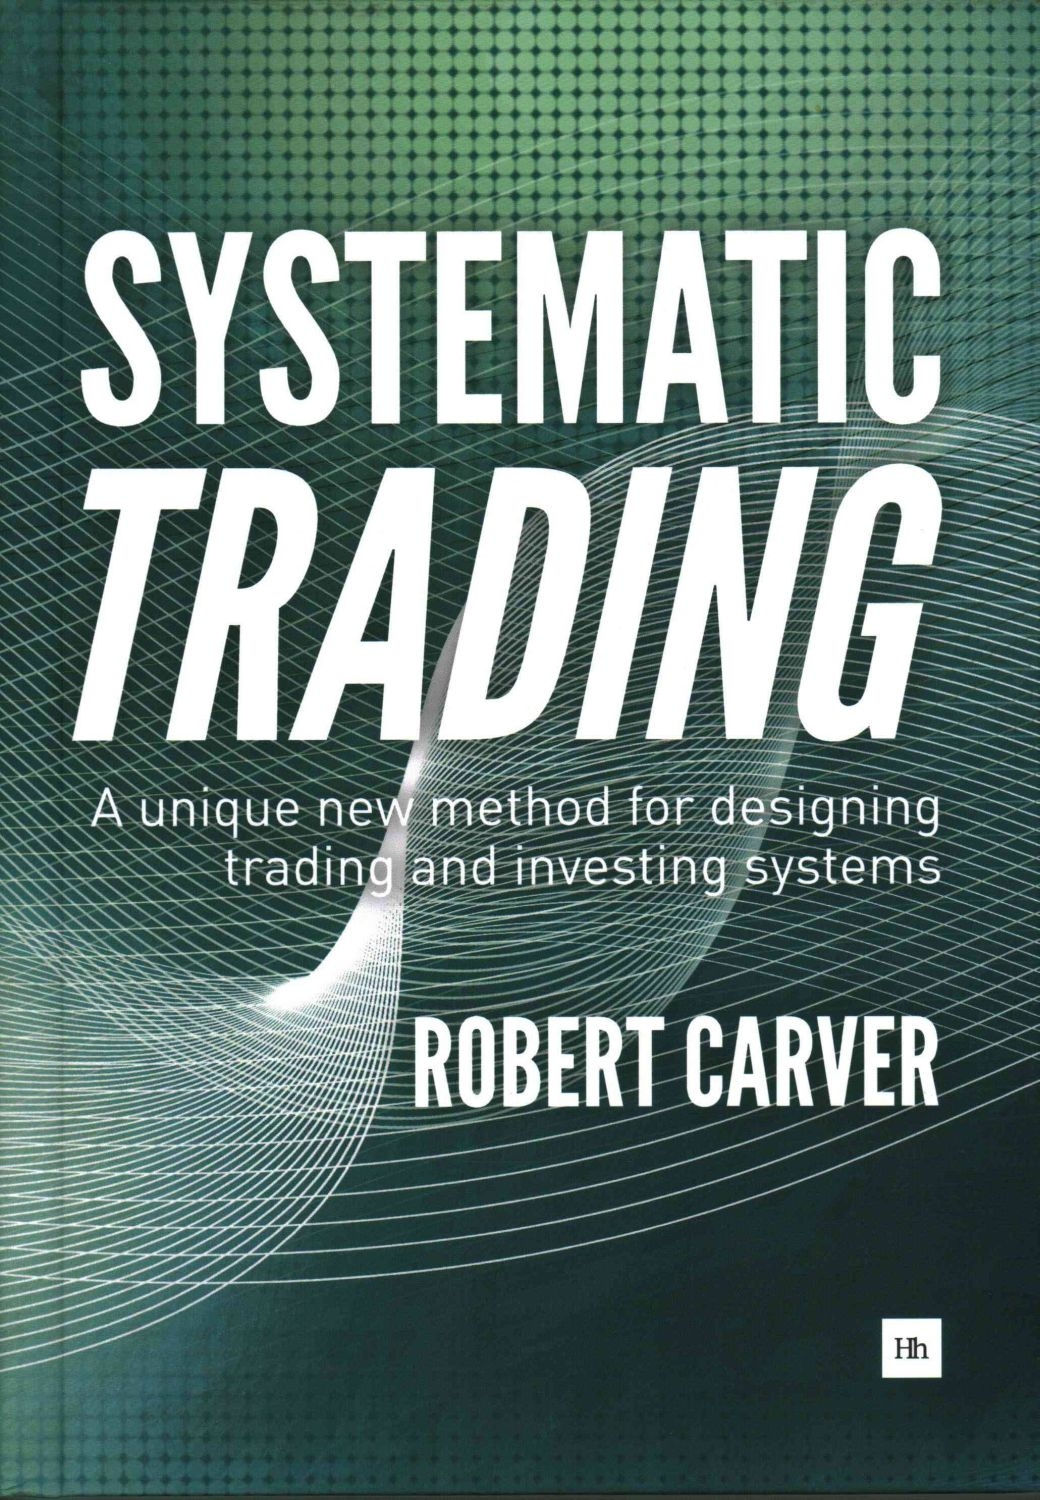
\includegraphics[width=\paperwidth,height=\paperheight]{figures/raw/img-000.jpg}%
};\end{tikzpicture}
\null \end{titlepage}

\thispagestyle{empty} \vspace*{0.12\textheight} \begin{center} {\bookdisplayfont\Huge\bfseries\englishdisplay{Systematic Trading} \par } \vspace{0.45em}
{\Large\bfseries\chinesedisplay{系统化交易}\par}
\end{center}

\vspace{1.6cm} \begin{center} \begin{tcolorbox}[enhanced, sharp corners, boxrule=0.5pt, colback=bookpaper, colframe=bookrule, width=0.74\textwidth, left=18pt, right=18pt, top=16pt, bottom=14pt] \raggedright \bookfrontlabel{About the Author}{作者简介}\small \begin{englishblock} Robert Carver worked in the City of London for over a decade. He initially traded exotic derivative products for Barclays Investment Bank and then worked as a portfolio manager for AHL --- one of the world's largest systematic hedge funds --- before, during and after the global financial meltdown of 2008. He was responsible for the creation of AHL's fundamental global macro strategy and then managed the fund's multi-billion dollar fixed income portfolio before retiring from the industry in 2013. Robert, who has bachelors and masters degrees in Economics, now systematically trades his own portfolio of futures and equities. \end{englishblock}

\vspace{1.0em} \begin{chineseblock}罗伯特·卡弗在伦敦金融城工作了十余年。起初，他在巴克莱投资银行交易各类奇异衍生品，随后加入 AHL担任投资组合经理。AHL 是全球最大的系统化对冲基金之一，而他在 2008 年全球金融危机爆发前、期间与之后都在该机构任职。他曾负责创建 AHL 的基本面全球宏观策略，之后又管理该基金规模达数十亿美元的固定收益投资组合，并于 2013 年退出行业。罗伯特拥有经济学学士和硕士学位，如今以系统化方式交易自己的期货和股票投资组合。\end{chineseblock}
\end{tcolorbox}

\vspace{1.15em} {\booksans\small\color{booksubtle}\englishdisplay{Robert Carver}\ {\color{bookrule}/}\ \chinesedisplay{罗伯特·卡弗} \par } \end{center}
\vfill

\clearpage \thispagestyle{empty} \vspace*{0.2\textheight} \begin{center} \begin{tcolorbox}[enhanced, sharp corners, boxrule=0.5pt, colback=bookpanel!68!bookpaper, colframe=bookrule, width=0.72\textwidth, left=18pt, right=18pt, top=18pt, bottom=18pt] \centering \bookfrontlabel{Complimentary eBook}{随书电子版}\small \englishdisplay{Every owner of a physical copy of this version of}\\[0.25em]
{\Large\bfseries\englishdisplay{Systematic Trading}}\\[0.25em]
\englishdisplay{can download the eBook for free direct from Harriman House,}\\
\englishdisplay{in a format that can be read on any eReader, tablet or smartphone.}\\[1.0em]
{\booksans\footnotesize\color{booksubtle}\englishdisplay{Download from}}\\[0.35em]
{\booksans\normalsize\bfseries\color{bookink}\url{ebooks.harriman-house.com/systematictrading}}\\[0.5em]
\englishdisplay{to get your free eBook now.}\\[1.35em]
\chinesedisplay{本版本《系统化交易》纸质书的每一位持有者，}\\
\chinesedisplay{都可以直接从 Harriman House 免费下载对应电子书版本，}\\
\chinesedisplay{并可在任意电子阅读器、平板电脑或智能手机上阅读。}\\[1.0em]
{\booksans\footnotesize\color{booksubtle}\chinesedisplay{下载地址}}\\[0.35em]
{\booksans\normalsize\bfseries\color{bookink}\url{ebooks.harriman-house.com/systematictrading}}\\[0.5em]
\chinesedisplay{即可立即获取你的免费电子书。}\end{tcolorbox}
\end{center}
\vfill

\clearpage \begin{titlepage} \thispagestyle{empty} \begin{center} \vspace*{0.17\textheight} {\booklabelcaps{Bilingual Edition} \par } \vspace{0.42em} {\booksans\normalsize\bfseries\chinesedisplay{中英双语版} \par } \vspace{1.65cm} {\bookdisplayfont\Huge\bfseries\englishdisplay{Systematic Trading} \par } \vspace{0.45em}
{\Large\bfseries\chinesedisplay{系统化交易}\par}
\vspace{1.3cm} \begin{minipage}{0.72\textwidth} \centering
{\Large\englishdisplay{A unique new method for designing trading\\and investing systems}\par}
\vspace{0.45em}
{\large\chinesedisplay{一种用于设计交易与投资系统的全新独特方法}\par}
\end{minipage}
\vspace{1.5em} \bookornament \vspace{2.0cm}
{\Large\englishdisplay{Robert Carver}\par}
\vspace{0.5em}
{\large\chinesedisplay{罗伯特·卡弗}\par}
\end{center}
\vfill \end{titlepage}
\thispagestyle{empty} \begingroup \scriptsize \setlength{\parindent}{0pt} \leftskip=0.11\textwidth \rightskip=0.11\textwidth \raggedright \vspace*{0.07\textheight} {\booklabelcaps{Publication Data} \par } \vspace{0.35em} {{\booksans\small\bfseries\chinesedisplay{版本信息} \par }} \vspace{0.65em} \bookminorornament \vspace{0.9em} \begin{englishblock} HARRIMAN HOUSE LTD\\
18 College Street\\
Petersfield\\
Hampshire\\
GU31 4AD\\
GREAT BRITAIN\\
Tel: +44 (0)1730 233870\\
Email: contact@harriman-house.com\\
Website: \url{www.harriman-house.com} \par \end{englishblock}

\vspace{0.65em} \begin{chineseblock}哈里曼出版社有限公司\\
英国汉普郡彼得斯菲尔德\\
学院街 18 号\\
邮编 GU31 4AD\\
电话：+44 (0)1730 233870\\
电子邮箱：contact@harriman-house.com\\
网站：\url{www.harriman-house.com} \par \end{chineseblock}

\vspace{0.8em} \begin{englishblock} First published in Great Britain in 2015\\
Copyright \copyright{} Robert Carver\\
The right of Robert Carver to be identified as the Author has been asserted in accordance with the Copyright, Designs and Patents Act 1988. \par \end{englishblock}

\vspace{0.65em} \begin{chineseblock}本书于 2015 年首次在英国出版。\\
版权 \copyright{} Robert Carver。\\
根据 1988 年《版权、外观设计与专利法》，罗伯特·卡弗作为本书作者的署名权已被正式主张并确认。 \par \end{chineseblock}

\vspace{0.8em} \begin{englishblock} Hardback ISBN: 9780857194459\\
eBook ISBN: 9780857195005 \par \end{englishblock}

\vspace{0.65em} \begin{chineseblock}精装本 ISBN：9780857194459\\
电子书 ISBN：9780857195005 \par \end{chineseblock}

\vspace{1.0em} \begin{englishblock} British Library Cataloguing in Publication Data\\
A CIP catalogue record for this book can be obtained from the British Library. \par \end{englishblock}

\vspace{0.65em} \begin{chineseblock}英国图书馆在版编目数据\\
本书的 CIP 编目记录可向英国图书馆索取。 \par \end{chineseblock}

\vspace{0.65em} \begin{englishblock} All rights reserved; no part of this publication may be reproduced, stored in a retrieval system, or transmitted in any form or by any means, electronic, mechanical, photocopying, recording, or otherwise without the prior written permission of the Publisher. This book may not be lent, resold, hired out or otherwise disposed of by way of trade in any form of binding or cover other than that in which it is published, without the prior written consent of the Publisher. \par \end{englishblock}

\vspace{0.65em} \begin{chineseblock}版权所有；未经出版方事先书面许可，本出版物的任何部分均不得以任何形式、通过任何方式复制、存储于检索系统，或进行传播，包括电子、机械、复印、录音等方式。未经出版方事先书面同意，本书不得以其出版形式之外的任何装帧或封面形式出借、转售、出租，或以其他贸易方式处分。 \par \end{chineseblock}

\vspace{0.65em} \begin{englishblock} No responsibility for loss occasioned to any person or corporate body acting or refraining to act as a result of reading material in this book can be accepted by the Publisher, by the Author, or by the Employer of the Author. \par \end{englishblock}

\vspace{0.65em} \begin{chineseblock}任何个人或机构因阅读本书内容而采取或不采取行动所造成的损失，出版方、作者及作者的雇主概不承担责任。 \par \end{chineseblock}

\vspace{0.85em} \begin{englishblock} Page number cross references refer to the print edition. \par \end{englishblock}

\vspace{0.65em} \begin{chineseblock}书中页码交叉引用均对应纸质版页码。
\par \end{chineseblock}
\endgroup \normalsize

\clearpage \thispagestyle{empty} \begin{center} \vspace*{0.25\textheight} \begin{minipage}{0.68\textwidth} \raggedright {\color{bookaccent!22}\fontsize{52}{52}\selectfont\bookdisplayfont`` \par } \vspace{-0.4em} \small \begin{englishblock} ``In every case the accuracy of experts was matched or exceeded by a simple algorithm... Why are experts inferior to algorithms? One reason... is that experts try to be clever, think outside the box, and consider complex combinations of features in making their predictions. Complexity may work in the odd case but more often than not it reduces validity.''\\[1.5em]
Daniel Kahneman, \textit{Thinking, Fast and Slow}\\[1.5em]
\end{englishblock}
\begin{chineseblock}“在每一种情况下，专家的准确性都与简单算法相当，甚至不如后者……为什么专家不如算法？其中一个原因……是专家总想耍聪明、跳出框架思考，并在做预测时考虑复杂的特征组合。复杂性在极少数情况下也许有效，但大多数时候它反而会降低有效性。”\\[1.5em]
丹尼尔·卡尼曼，\textit{Thinking, Fast and Slow} \end{chineseblock}
\vspace{0.9em} \bookornament \end{minipage}
\end{center}

\endgroup
